\documentclass[12pt,a4paper]{article}

% Pakiety
\usepackage[utf8]{inputenc}
\usepackage[polish]{babel}
\usepackage[T1]{fontenc}
\usepackage{graphicx}
\usepackage{booktabs}
\usepackage{amsmath}
\usepackage{amssymb}
\usepackage{hyperref}
\usepackage{caption}
\usepackage{subcaption}
\usepackage{float}
\usepackage{geometry}
\usepackage{fancyhdr}
\usepackage{setspace}

% Ustawienia strony
\geometry{
    left=2.5cm,
    right=2.5cm,
    top=2.5cm,
    bottom=2.5cm
}

% Ustawienia odstepow
\onehalfspacing

% Sciezka do grafik
\graphicspath{{figures/}{../experiments/results/}}

% Wszystkie float w dokladnym miejscu
\floatplacement{figure}{H}
\floatplacement{table}{H}

% Informacje o dokumencie
\title{%
    {\Large\textbf{Przewidywanie Dlugosci Pobytu w Szpitalu\\
    za pomoca Sieci Neuronowych}}\\[0.5cm]
    {\large Projekt z Sieci Neuronowych i Uczenia Glebokiego}
}

\author{%
    [Imie i Nazwisko]\\
    [Numer indeksu]\\
    [Wydzial]\\
    [Uniwersytet]
}

\date{\today}

% Numeracja sekcji
\setcounter{secnumdepth}{3}
\setcounter{tocdepth}{3}

\begin{document}

% Title page
\maketitle
\thispagestyle{empty}

\newpage

% Spis tresci
\tableofcontents
\newpage

% Sekcje
\section{Wprowadzenie}

\subsection{Sformułowanie problemu}

Długość pobytu w szpitalu jest kluczowym wskaźnikiem w zarządzaniu służbą zdrowia. Dokładne przewidywanie czasu hospitalizacji pozwala na optymalizację wykorzystania łóżek szpitalnych, lepsze planowanie personelu oraz skuteczniejsze zarządzanie kosztami.

Problem przewidywania długości pobytu stanowi zadanie \textbf{regresji}, w którym na podstawie czynników ryzyka zdrowotnego pacjenta należy oszacować liczbę dni hospitalizacji.

\subsection{Cel projektu}

Celem projektu jest opracowanie i ocena modeli sieci neuronowych przewidujących długość pobytu w szpitalu na podstawie danych Healthcare Risk Factors Dataset. Projekt obejmuje przygotowanie danych, implementację trzech architektur (SimpleMLP, TabNet, TabTransformer), systematyczne przeszukiwanie hiperparametrów oraz wybór najlepszego modelu.

\subsection{Wykorzystane metody}

Zastosowano trzy architektury sieci neuronowych dostosowane do danych tabelarycznych:

\begin{itemize}
    \item \textbf{SimpleMLP} -- klasyczna architektura fully-connected (baseline)
    \item \textbf{TabNet} -- architektura z mechanizmem attention i selekcją cech
    \item \textbf{TabTransformer} -- architektura oparta na mechanizmie Transformer
\end{itemize}

\newpage

\section{Dane}

\subsection{Opis zbioru danych}

W projekcie wykorzystano zbiór danych \textit{Healthcare Risk Factors Dataset}, dostępny publicznie na platformie Kaggle \cite{healthcare_dataset}. Zbiór zawiera informacje o pacjentach oraz czynnikach ryzyka zdrowotnego, które mogą wpływać na długość ich pobytu w szpitalu.

Oryginalny zbiór danych zawierał następujące informacje:
\begin{itemize}
    \item Dane demograficzne (wiek, płeć)
    \item Czynniki fizjologiczne (BMI, ciśnienie krwi, poziom cholesterolu)
    \item Czynniki behawioralne (palenie, aktywność fizyczna)
    \item Diagnozę medyczną (stan zdrowia, choroby przewlekłe)
    \item Długość pobytu w szpitalu (zmienna docelowa)
\end{itemize}

\subsection{Preprocessing danych}

Dane wymagały przeprowadzenia szeregu operacji przygotowawczych w celu uzyskania formatu odpowiedniego dla trenowania sieci neuronowych:

\subsubsection{Usunięcie kolumn szumu}

Zbiór danych zawierał celowo wprowadzone kolumny szumu służące do testowania algorytmów selekcji cech:
\begin{itemize}
    \item \texttt{random\_notes} -- losowe notatki tekstowe
    \item \texttt{noise\_col} -- kolumna z wartościami losowymi
\end{itemize}

Kolumny te zostały usunięte przed dalszym przetwarzaniem, gdyż nie niosły żadnej informacji predykcyjnej.

\subsubsection{Obsługa brakujących danych}

Zbiór danych zawierał pewną liczbę rekordów z brakującymi wartościami. Ze względu na stosunkowo niewielką liczbę takich przypadków oraz chęć uniknięcia wprowadzania błędów systematycznych przez imputację, zdecydowano się na usunięcie wierszy zawierających wartości \texttt{NaN}. Analiza wykazała, że liczba usuniętych rekordów była minimalna i nie wpływała negatywnie na reprezentatywność zbioru.

\subsubsection{Kodowanie zmiennych kategorycznych}

Zbiór danych zawierał dwie zmienne kategoryczne wymagające numerycznego zakodowania:

\textbf{Płeć (Gender):}
\begin{itemize}
    \item \texttt{Male} → 1
    \item \texttt{Female} → 0
\end{itemize}

\textbf{Stan medyczny (Medical Condition):}\\
Zmienna kategoryczna reprezentująca różne stany zdrowia pacjentów została zakodowana przy użyciu metody one-hot encoding. Dla każdego unikalnego stanu medycznego (z wyjątkiem \texttt{Healthy}) utworzono osobną kolumnę binarną:

\begin{itemize}
    \item Jeśli pacjent ma dany stan medyczny, wartość kolumny = 1
    \item W przeciwnym wypadku wartość kolumny = 0
    \item Pacjenci oznaczeni jako \texttt{Healthy} mają wartość 0 we wszystkich kolumnach stanów medycznych
\end{itemize}

Po zakodowaniu oryginalna kolumna \texttt{Medical Condition} została usunięta.

\subsection{Podział danych}

Dane zostały podzielone na zbiór treningowy i testowy w proporcji:
\begin{itemize}
    \item \textbf{Zbiór treningowy}: 80\% danych
    \item \textbf{Zbiór testowy}: 20\% danych
\end{itemize}

Podział został wykonany z użyciem \texttt{random\_state=42} w celu zapewnienia reprodukowalności wyników. Zbiór treningowy został wykorzystany do przeprowadzenia walidacji krzyżowej oraz treningu modeli, natomiast zbiór testowy pozostał niewidoczny dla modeli podczas całego procesu optymalizacji i został użyty wyłącznie do końcowej oceny wybranego najlepszego modelu.

\subsection{Statystyki danych}

Finalny zbiór danych:
\begin{itemize}
    \item \textbf{Liczba cech}: 22
    \item \textbf{Zmienna docelowa}: Długość pobytu w dniach
    \item \textbf{Podział}: 80\% trening, 20\% test
\end{itemize}

\newpage

\section{Metodyka}

Proces optymalizacji modeli obejmował grid search z 5-fold cross-validation, early stopping oraz ocenę na zbiorze testowym.

\subsection{Grid Search}

Grid Search (przeszukiwanie siatki) to metoda systematycznego przeszukiwania przestrzeni hiperparametrów poprzez wytrenowanie i ocenę modelu dla każdej możliwej kombinacji wartości hiperparametrów ze zdefiniowanej siatki.

\subsubsection{Przestrzeń hiperparametrów}

Dla każdej architektury zdefiniowano specyficzną przestrzeń hiperparametrów:

\begin{itemize}
    \item \textbf{SimpleMLP}: 3 × 2 × 3 = 18 możliwych konfiguracji
    \begin{itemize}
        \item \texttt{hidden\_channels}: [64, 128, 256]
        \item \texttt{activation\_layer}: ['relu', 'tanh']
        \item \texttt{dropout}: [0.2, 0.3, 0.4]
    \end{itemize}
    
    \item \textbf{TabNet}: 3 × 3 × 3 = 27 możliwych konfiguracji
    \begin{itemize}
        \item \texttt{n\_d}: [8, 32, 64]
        \item \texttt{n\_a}: [8, 32, 64]
        \item \texttt{n\_steps}: [3, 5, 7]
    \end{itemize}
    
    \item \textbf{TabTransformer}: 3 × 3 × 3 = 27 możliwych konfiguracji
    \begin{itemize}
        \item \texttt{d\_model}: [64, 128, 256]
        \item \texttt{n\_heads}: [2, 4, 8]
        \item \texttt{num\_layers}: [1, 2, 3]
    \end{itemize}
\end{itemize}

Szczegółowe opisy hiperparametrów znajdują się w sekcji \ref{sec:architectures}.

\subsection{Walidacja krzyżowa i early stopping}

Zastosowano 5-fold cross-validation z early stopping (patience=10 epok, max 100 epok). Każda konfiguracja była trenowana 5 razy z różnymi podziałami danych, a metryki uśredniano.

\subsection{Metryki oceny}

Wykorzystano standardowe metryki regresji: MAE, RMSE, R², MAPE oraz MedAE.

\subsection{Optymalizacja}

Modele trenowano przy użyciu optymalizatora Adam (learning rate: 0.001 dla MLP i TabTransformer, 0.02 dla TabNet) z funkcją straty L1Loss (MAE).

\newpage

\section{Architektury Modeli}
\label{sec:architectures}

W projekcie zaimplementowano i porównano trzy różne architektury sieci neuronowych, każda z unikalnymi cechami dostosowanymi do pracy z danymi tabelarycznymi.

\subsection{SimpleMLP}

Klasyczna architektura fully-connected: warstwa wejściowa (22 cechy) → warstwa ukryta → dropout → warstwa wyjściowa.

\begin{table}[h]
\centering
\caption{Przestrzeń hiperparametrów dla MLP}
\label{tab:hyperparams_mlp}
\begin{tabular}{lll}
\toprule
Hiperparametr & Wartości & Opis \\
\midrule
hidden\_channels & [64, 128, 256] & Liczba neuronów w warstwie ukrytej \\
activation\_layer & ['relu', 'tanh'] & Funkcja aktywacji \\
dropout & [0.2, 0.3, 0.4] & Współczynnik dropout \\
\bottomrule
\end{tabular}
\end{table}


\subsection{TabNet}

Specjalizowana architektura wykorzystująca mechanizm attention do sekwencyjnej selekcji cech \cite{arik2019tabnet}. Oferuje interpretowalność poprzez maski attention pokazujące istotność cech.

\begin{table}[h]
\centering
\caption{Przestrzeń hiperparametrów dla TABNET}
\label{tab:hyperparams_tabnet}
\begin{tabular}{lll}
\toprule
Hiperparametr & Wartości & Opis \\
\midrule
n\_d & [8, 32, 64] & Wymiar feature transformers \\
n\_a & [8, 32, 64] & Wymiar attention layers \\
n\_steps & [3, 5, 7] & Liczba kroków decyzyjnych \\
\bottomrule
\end{tabular}
\end{table}


\subsection{TabTransformer}

Architektura oparta na mechanizmie Transformer \cite{vaswani2017attention}, wykorzystująca self-attention do modelowania zależności między cechami.

\begin{table}[h]
\centering
\caption{Przestrzeń hiperparametrów dla TABTRANSFORMER}
\label{tab:hyperparams_tabtransformer}
\begin{tabular}{lll}
\toprule
Hiperparametr & Wartości & Opis \\
\midrule
d\_model & [64, 128, 256] & Wymiar modelu \\
n\_heads & [2, 4, 8] & Liczba głów attention \\
num\_layers & [1, 2, 3] & Liczba warstw transformera \\
\bottomrule
\end{tabular}
\end{table}


\newpage

\section{Proces Treningu}

Dla każdej konfiguracji hiperparametrów przeprowadzono 5-fold cross-validation z early stopping. Najlepsze modele wybrano na podstawie średniego MAE z walidacji. Wygenerowano wykresy predykcji, reszt oraz Q-Q plots dla oceny jakości modeli.

\newpage

\section{Wyniki Eksperymentów}

Dla każdej architektury przeprowadzono grid search z 5-fold cross-validation.

\subsection{Porównanie architektur}

\begin{figure}[H]
\centering
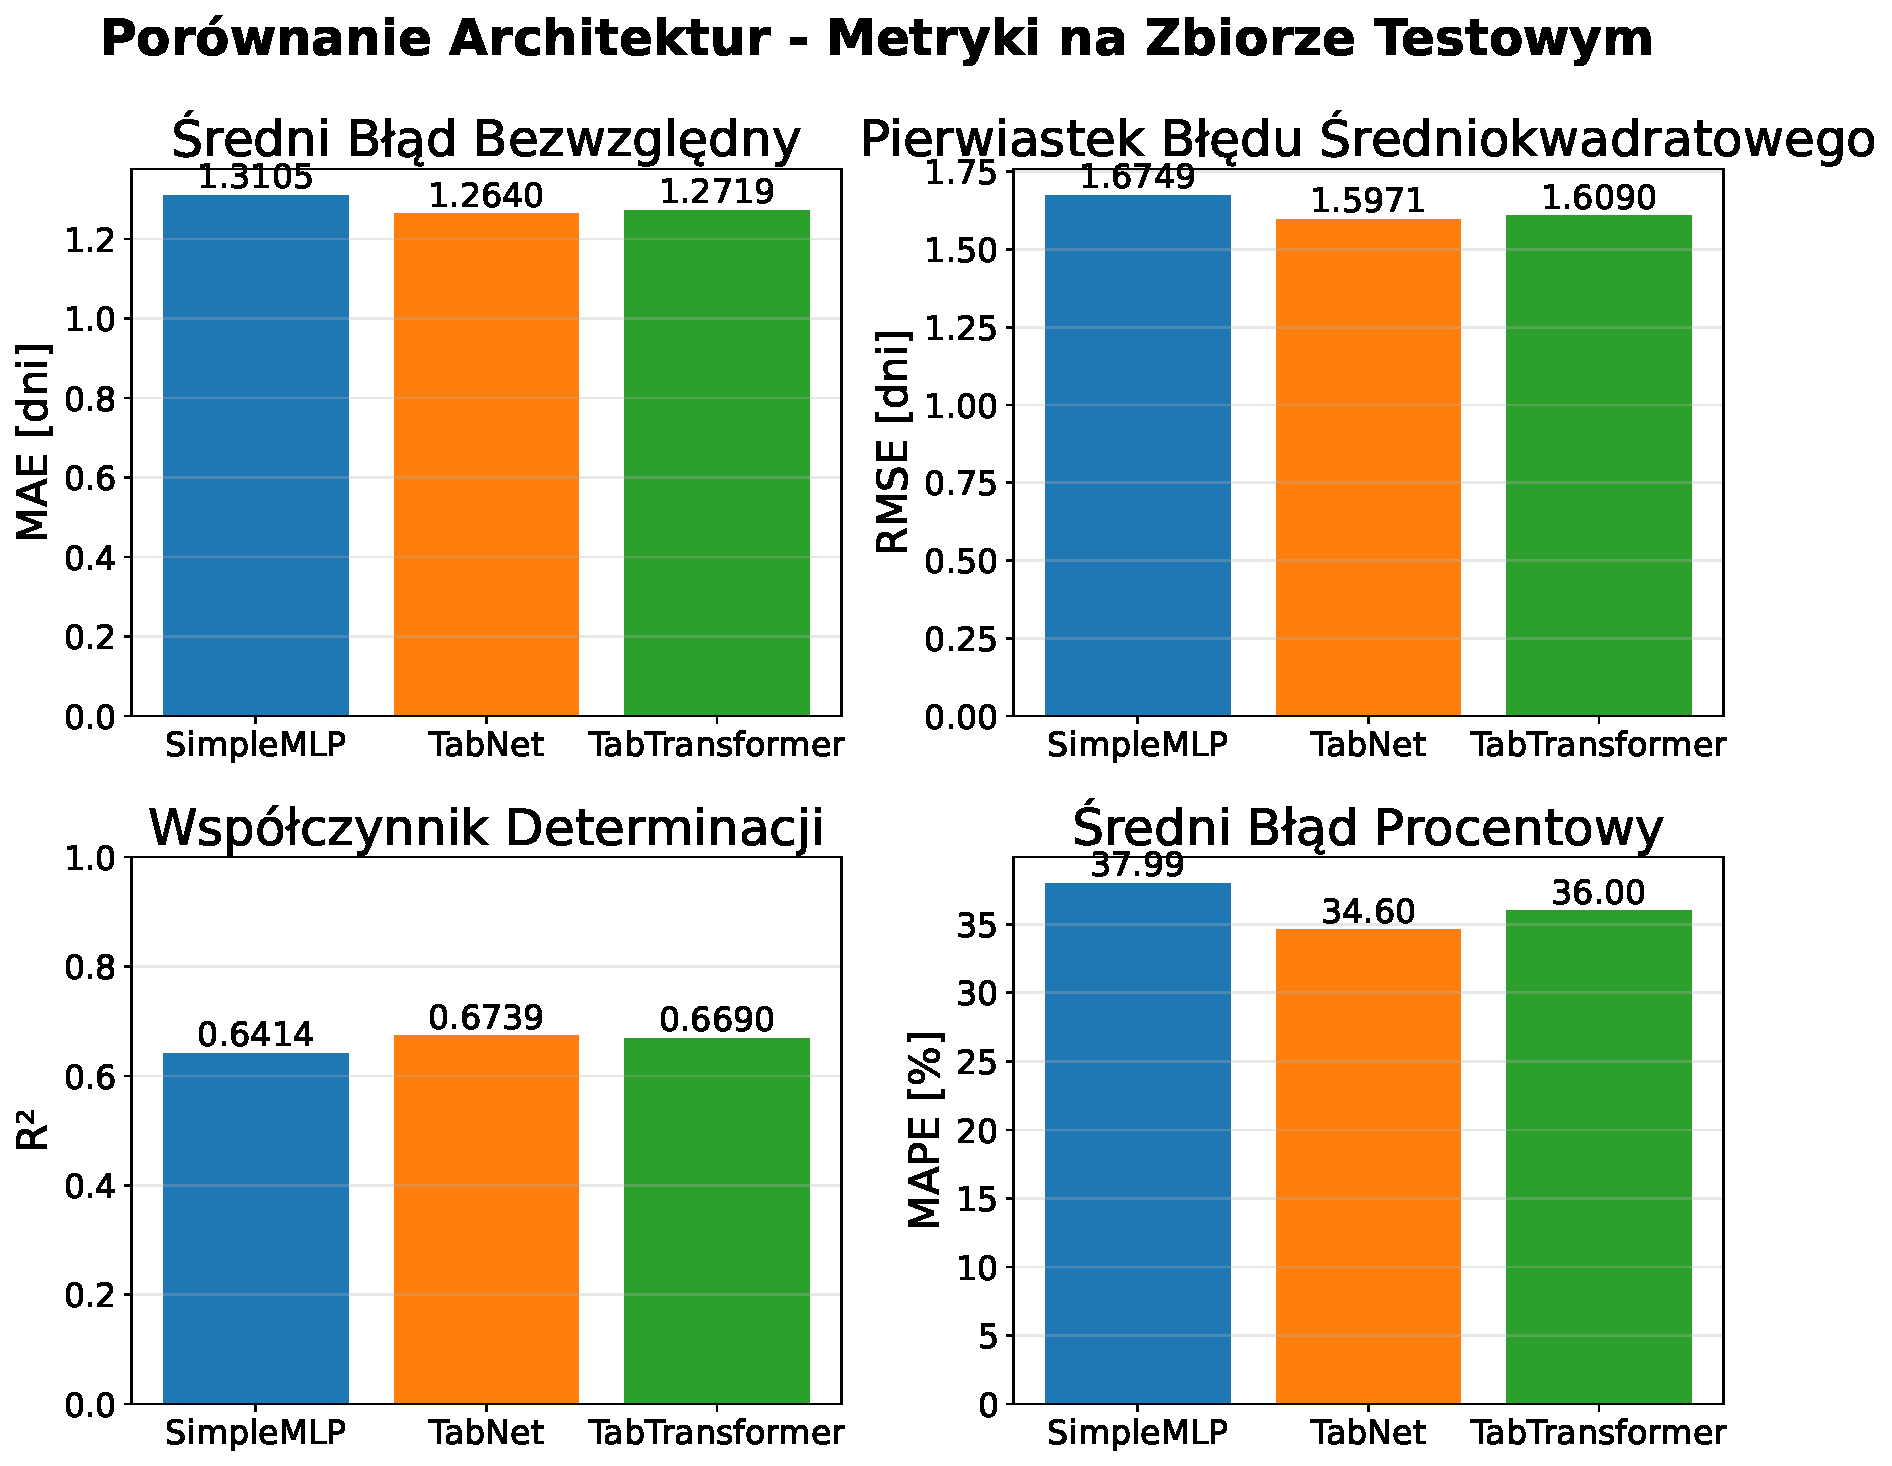
\includegraphics[width=0.95\textwidth]{figures/architecture_comparison.pdf}
\caption{Porównanie architektur - metryki testowe}
\end{figure}

\begin{figure}[H]
\centering
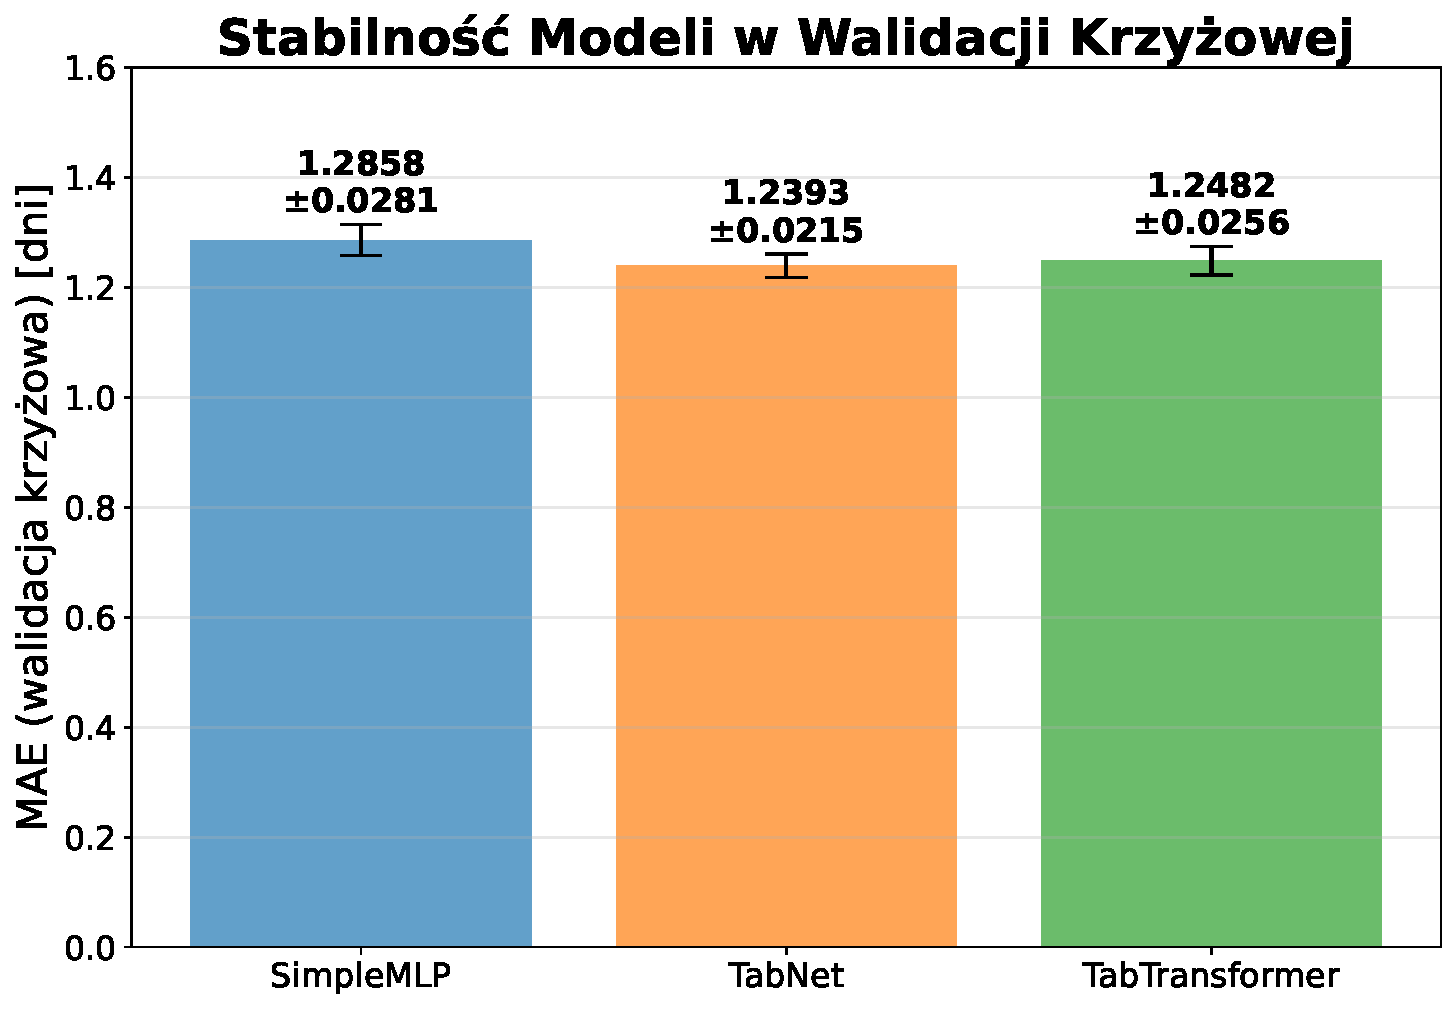
\includegraphics[width=0.75\textwidth]{figures/cv_stability.pdf}
\caption{Stabilność modeli w walidacji krzyżowej}
\end{figure}

TabNet osiągnął najlepsze wyniki we wszystkich metrykach.

\subsection{SimpleMLP}

\begin{table}[H]
\centering
\caption{Najlepszy model SimpleMLP}
\begin{tabular}{lc}
\toprule
Parametr & Wartość \\
\midrule
Hidden features & 256 \\
Dropout & 0.2 \\
Activation & ReLU \\
MAE (CV) & 1.2858 $\pm$ 0.0281 \\
MAE (Test) & 1.3105 \\
R² (Test) & 0.6414 \\
\bottomrule
\end{tabular}
\end{table}

\subsection{TabNet}

\begin{table}[H]
\centering
\caption{Najlepszy model TabNet}
\begin{tabular}{lc}
\toprule
Parametr & Wartość \\
\midrule
n\_d & 64 \\
n\_a & 32 \\
n\_steps & 3 \\
MAE (CV) & 1.2393 $\pm$ 0.0215 \\
MAE (Test) & \textbf{1.2640} \\
R² (Test) & \textbf{0.6739} \\
\bottomrule
\end{tabular}
\end{table}

\subsection{TabTransformer}

\begin{table}[H]
\centering
\caption{Najlepszy model TabTransformer}
\begin{tabular}{lc}
\toprule
Parametr & Wartość \\
\midrule
d\_model & 128 \\
n\_heads & 2 \\
num\_layers & 2 \\
MAE (CV) & 1.2482 $\pm$ 0.0256 \\
MAE (Test) & 1.2719 \\
R² (Test) & 0.6690 \\
\bottomrule
\end{tabular}
\end{table}

\newpage

\section{Szczegółowa analiza najlepszych modeli}

\subsection{SimpleMLP}

\begin{figure}[H]
\centering
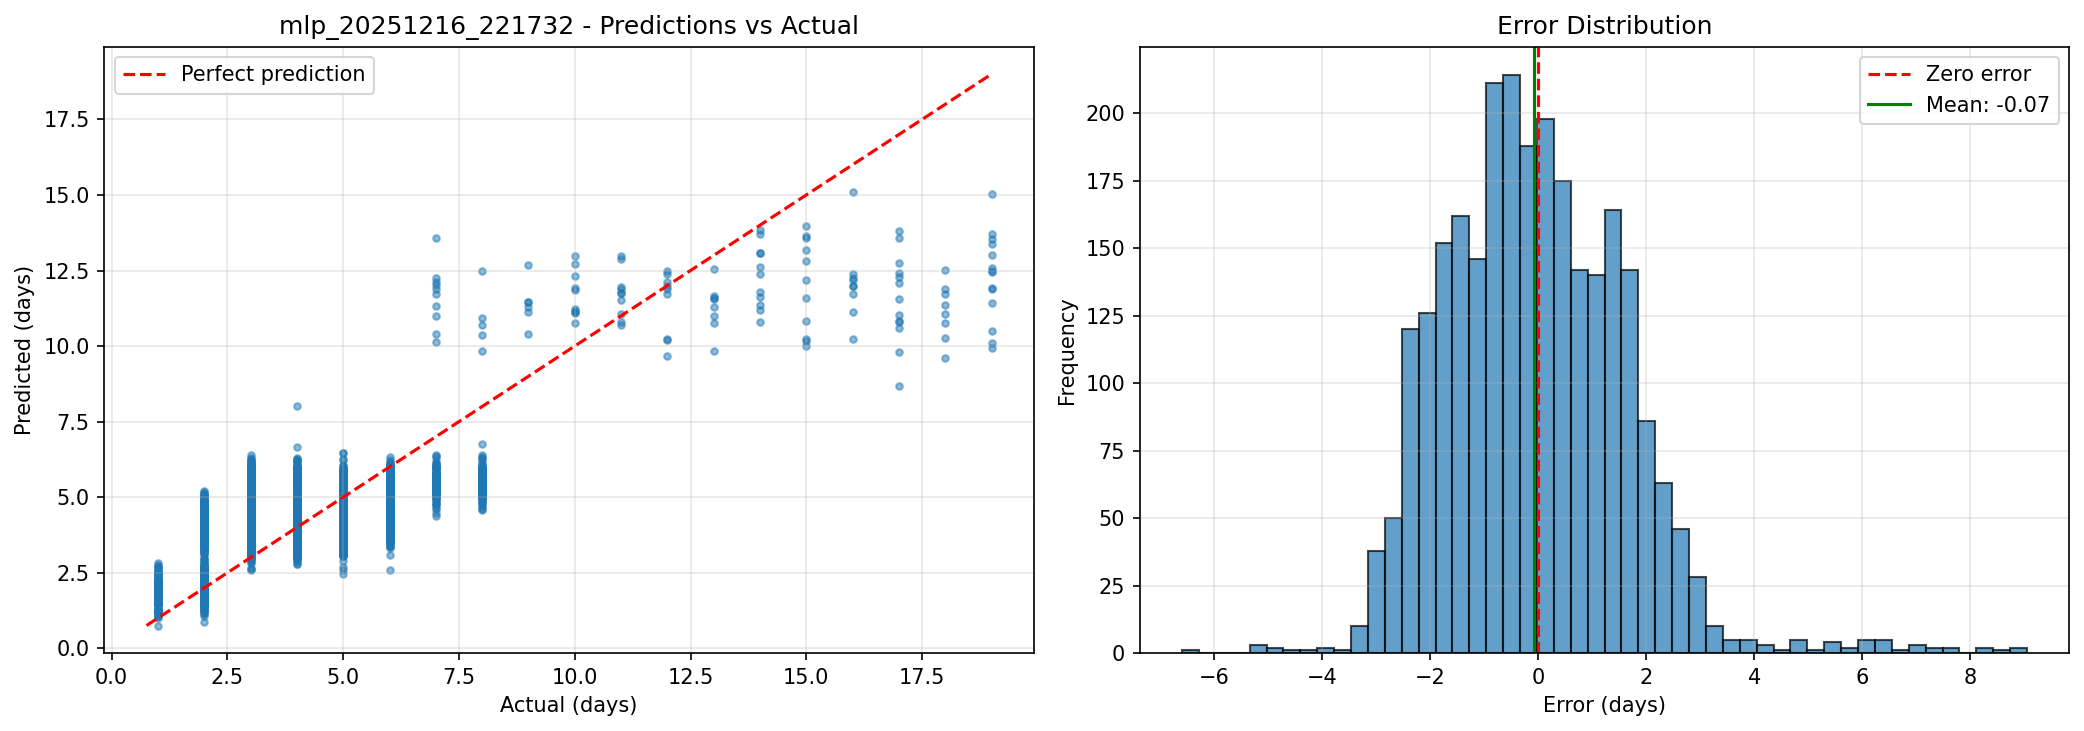
\includegraphics[width=0.45\textwidth]{figures/mlp_predictions.pdf}
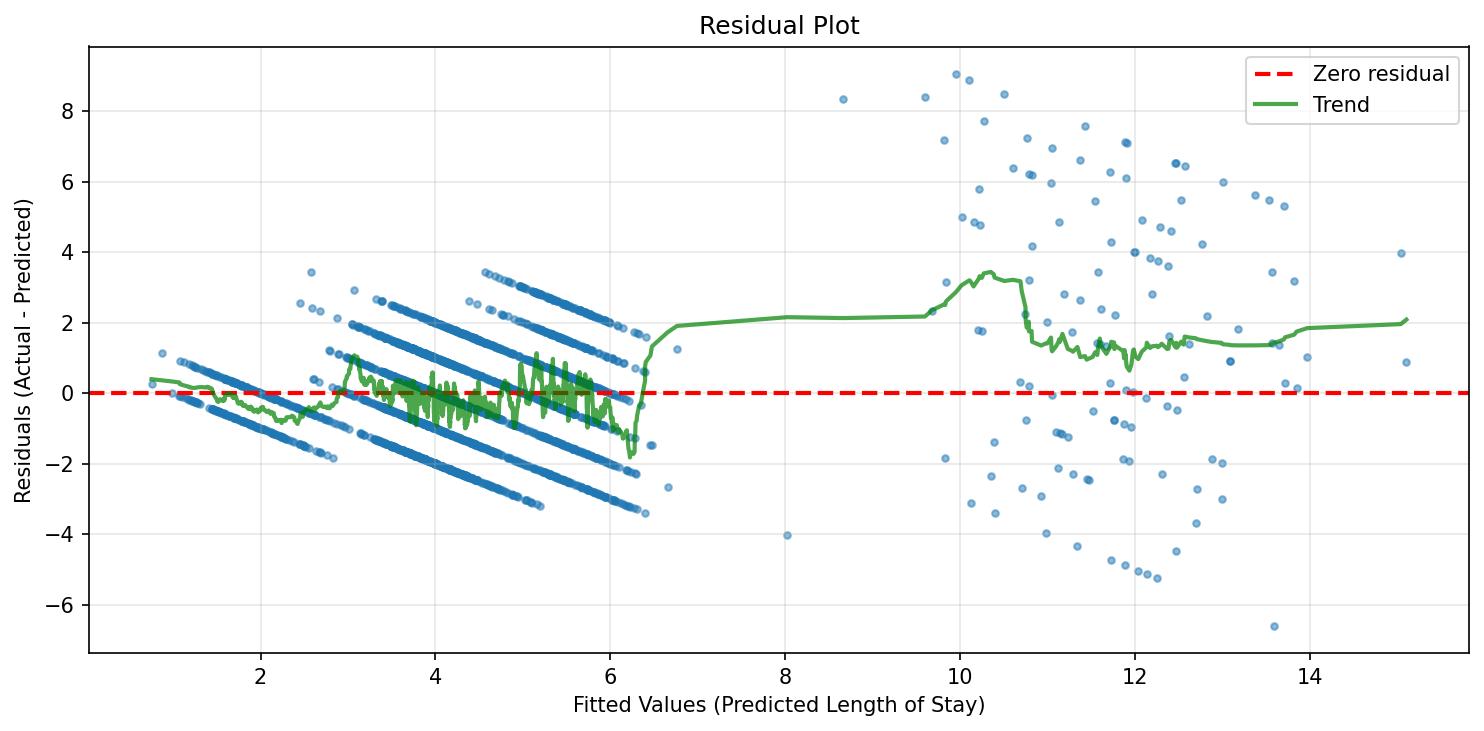
\includegraphics[width=0.45\textwidth]{figures/mlp_residuals.pdf}
\caption{Predykcje i reszty dla SimpleMLP}
\end{figure}

Model wykazał dobr ą korelację między predykcjami a wartościami rzeczywistymi. Reszty są losowo rozłożone z tendencją do większych błędów dla długich pobytów.

\subsection{TabNet}

\begin{figure}[H]
\centering
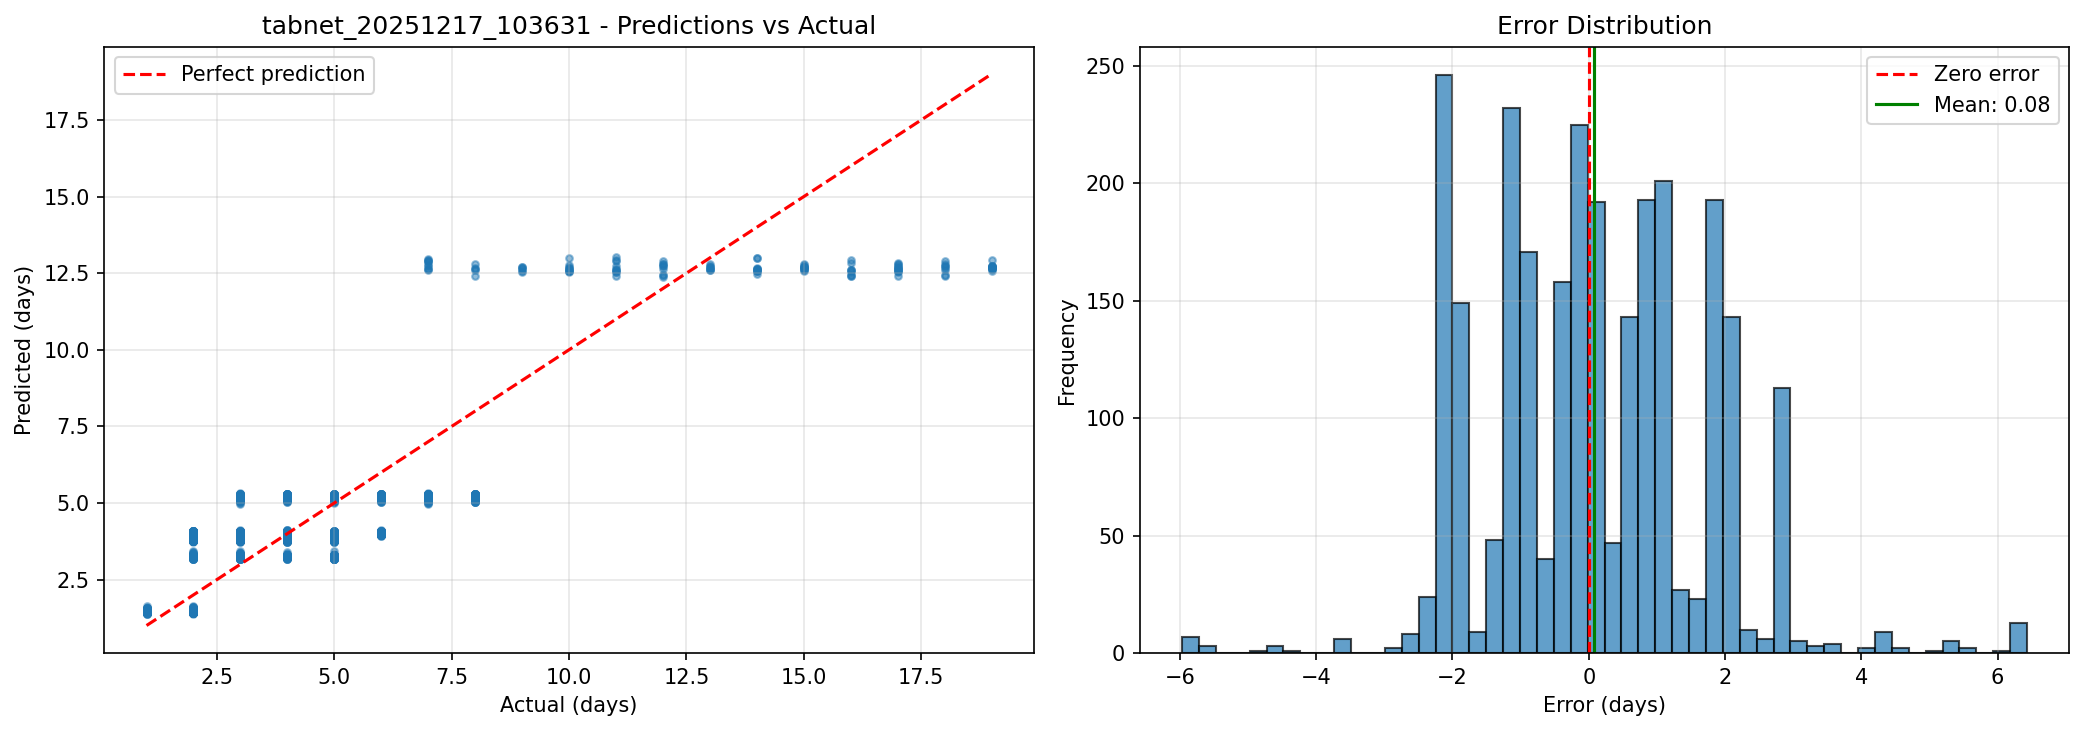
\includegraphics[width=0.45\textwidth]{figures/tabnet_predictions.pdf}
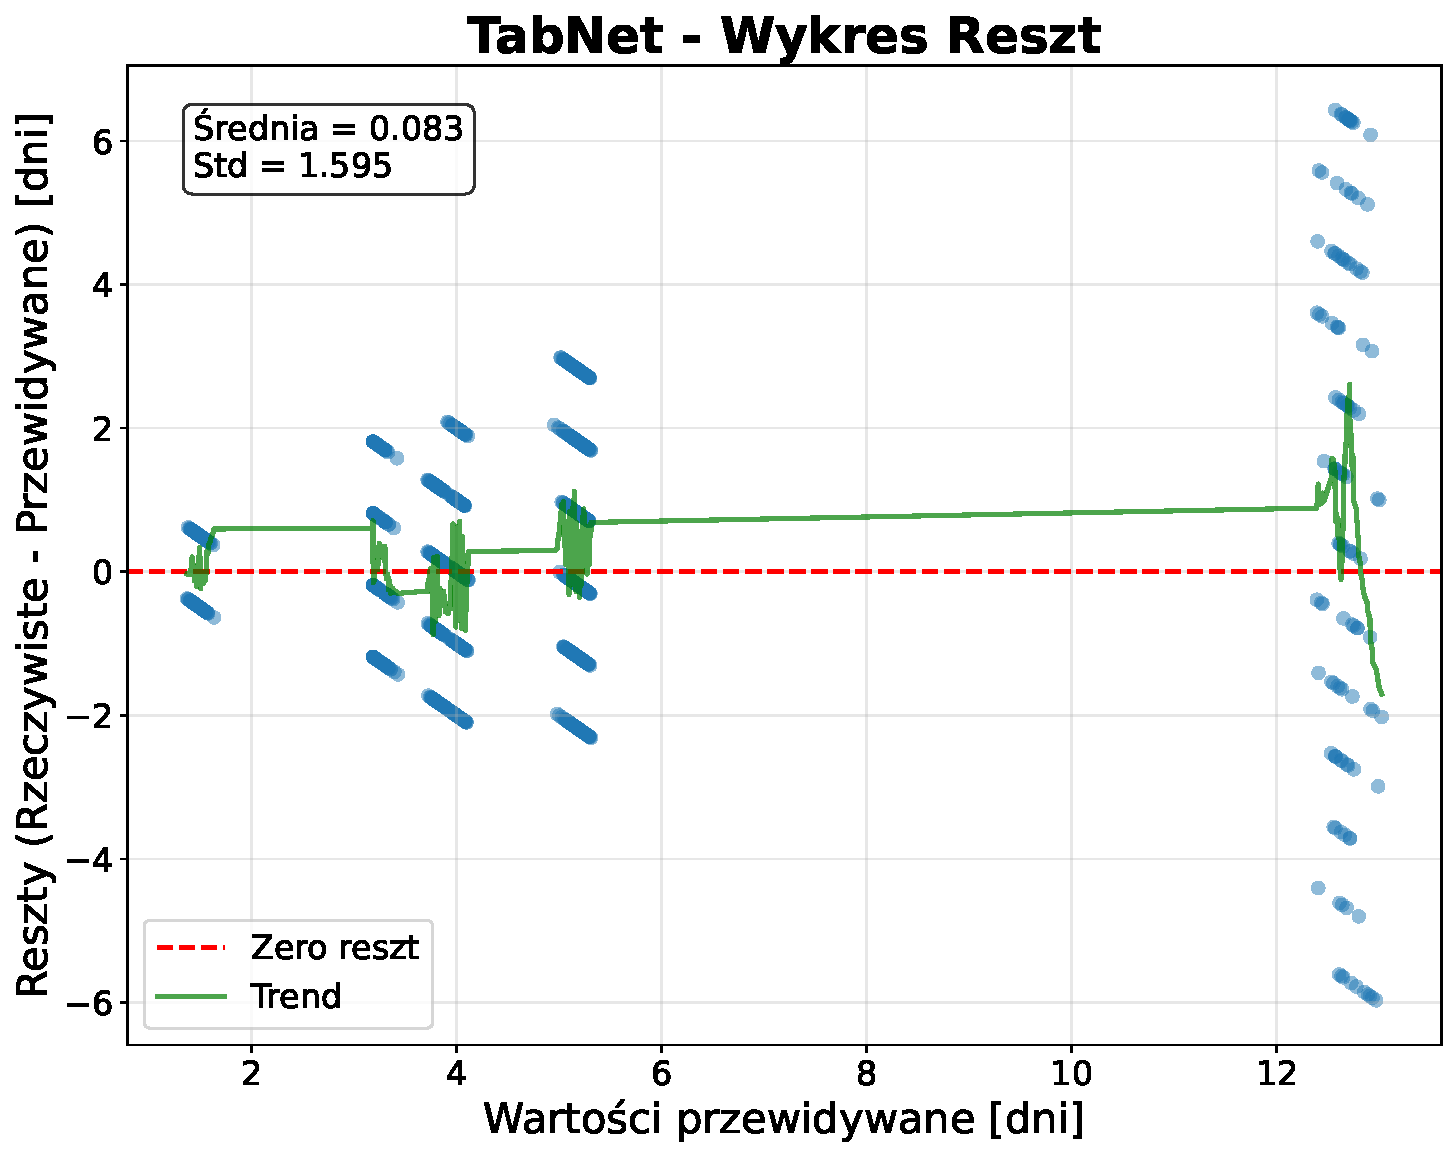
\includegraphics[width=0.45\textwidth]{figures/tabnet_residuals.pdf}
\caption{Predykcje i reszty dla TabNet}
\end{figure}

Najlepsze dopasowanie ze wszystkich modeli. Równomierne rozproszenie reszt wskazuje na homoskedastyczność. Mechanizm attention pozwala na interpretację decyzji modelu.

\subsection{TabTransformer}

\begin{figure}[H]
\centering
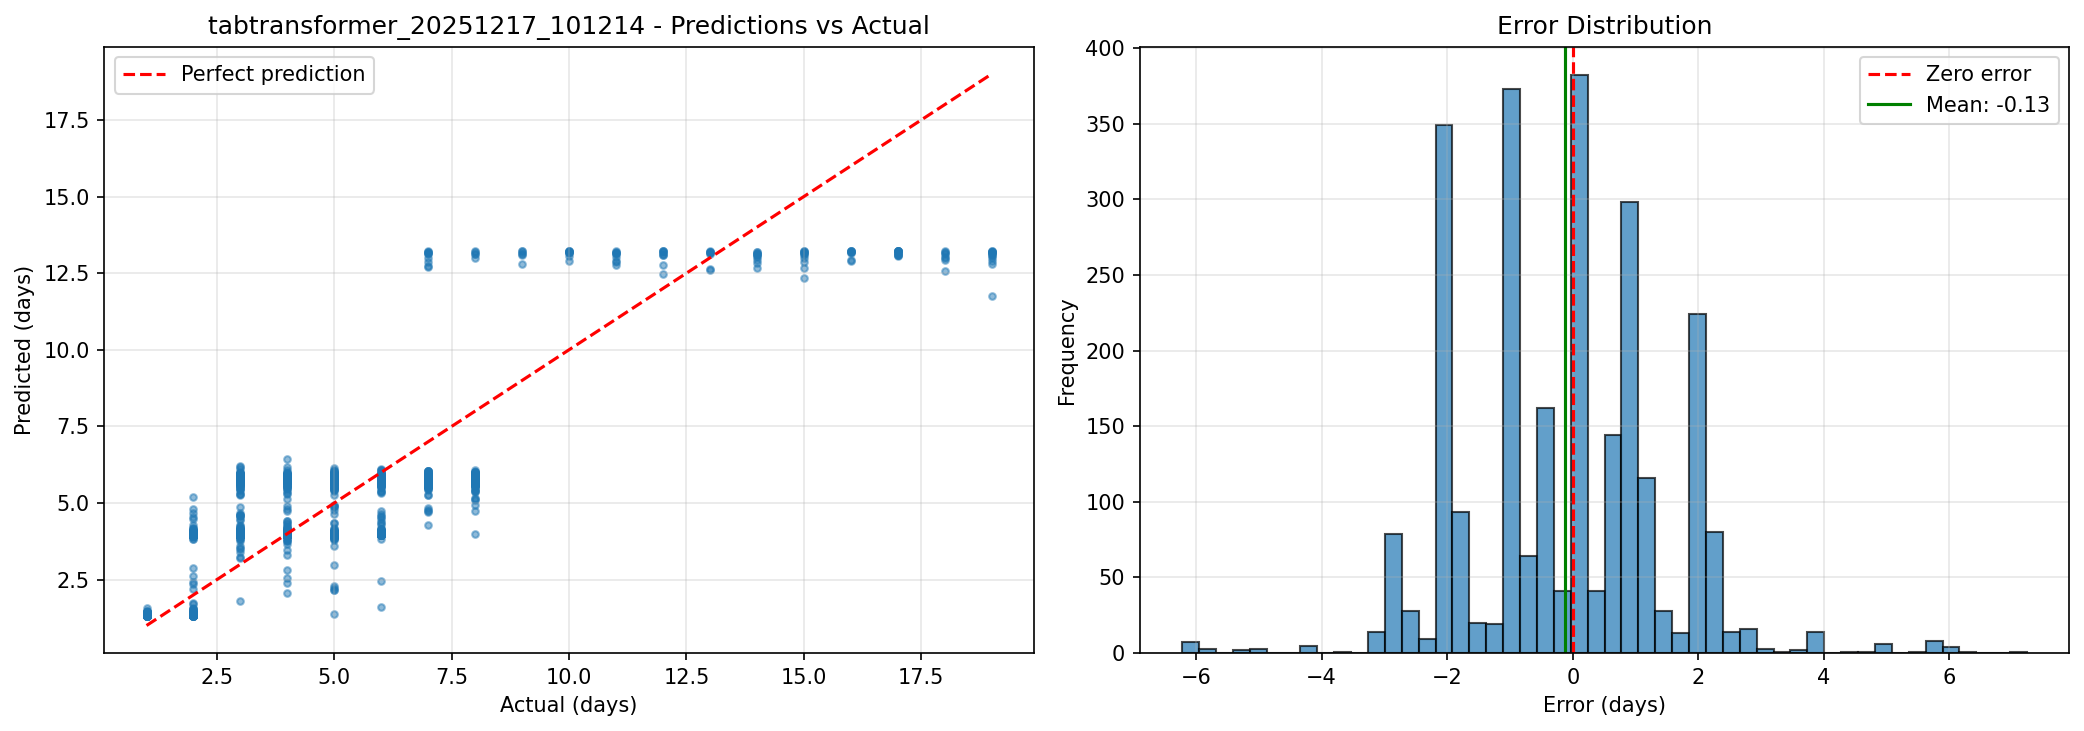
\includegraphics[width=0.45\textwidth]{figures/tabtransformer_predictions.pdf}
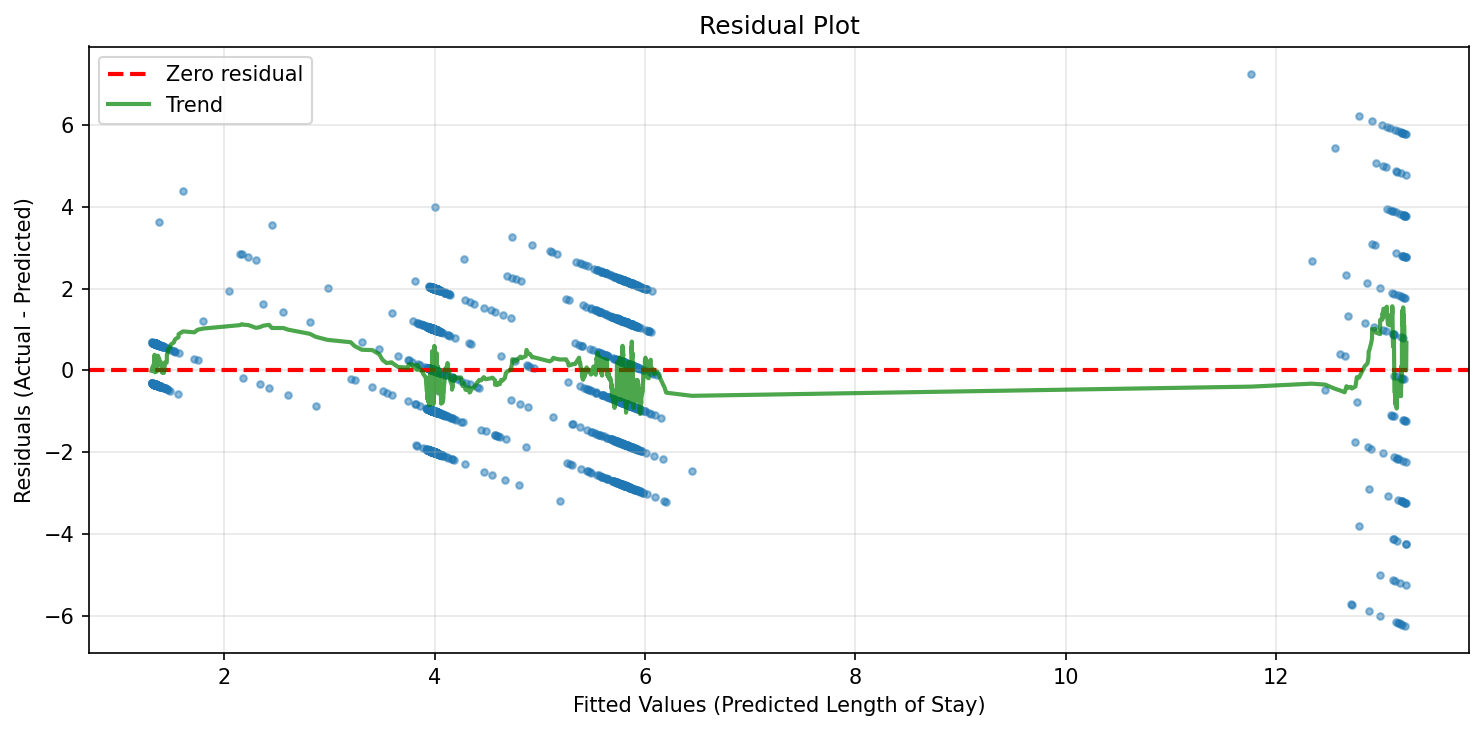
\includegraphics[width=0.45\textwidth]{figures/tabtransformer_residuals.pdf}
\caption{Predykcje i reszty dla TabTransformer}
\end{figure}

Bardzo dobre dopasowanie, porównywalne z TabNet. Stabilna wariancja reszt w całym zakresie wartości.

\newpage

\section{Końcowa analiza najlepszego modelu}

\textbf{TabNet} został wybrany jako najlepszy model ze względu na:

\begin{itemize}
    \item Najniższy MAE (1.2640 dni) i RMSE (1.5971 dni)
    \item Najwyższy R² (0.6739) -- wyjaśnia 67\% wariancji
    \item Wyjątkową stabilność (std MAE = 0.0006 dni)
    \item Wbudowaną interpretowalność (feature importance)
\end{itemize}

\subsection{Mocne strony}

\begin{itemize}
    \item Najwyższa dokładność predykcyjna
    \item Minimalna zmienność między foldami CV
    \item Mechanizm attention umożliwia identyfikację istotnych cech
    \item Najniższy maksymalny błąd (6.43 dni vs 9.05 dla MLP)
\end{itemize}

\subsection{Ograniczenia}

\begin{itemize}
    \item Trudności z ekstremalnymi czasami pobytu (>10 dni)
    \item 33\% niewytłumaczonej wariancji
    \item Brak przedziałów ufności dla predykcji
\end{itemize}

\subsection{Poprawa względem baseline}

\begin{table}[H]
\centering
\caption{Poprawa TabNet względem SimpleMLP}
\begin{tabular}{lrrr}
\toprule
Metryka & SimpleMLP & TabNet & Poprawa \\
\midrule
MAE & 1.3105 & 1.2640 & -3.55\% \\
RMSE & 1.6749 & 1.5971 & -4.64\% \\
R² & 0.6414 & 0.6739 & +5.07\% \\
Max Error & 9.0501 & 6.4306 & -28.94\% \\
\bottomrule
\end{tabular}
\end{table}

Model jest gotowy do wdrożenia jako narzędzie wspomagające planowanie zarządzania zasobami szpitalnymi.

\newpage

\section{Wnioski}

\subsection{Podsumowanie wyników}

Projekt zrealizował cel przewidywania długości pobytu w szpitalu. Przetestowano 3 architektury (SimpleMLP, TabNet, TabTransformer) z łącznie 62 konfiguracjami. Wszystkie modele osiągnęły R² powyżej 0.64.

Najlepszy model (TabNet): MAE = 1.26 dnia, R² = 0.67.

\subsection{Stosowalność rozwiązania}

Model może wspierać:
\begin{itemize}
    \item Planowanie wykorzystania łóżek szpitalnych
    \item Optymalizację zarządzania personelem
    \item Analizę kosztów i budżetowanie
\end{itemize}

Model powinien wspomagać, nie zastępować osąd medyczny.

\subsection{Ograniczenia}

\begin{itemize}
    \item Ograniczona liczba cech (22)
    \item Trudności z ekstremalnymi czasami pobytu
    \item 33\% niewytłumaczonej wariancji
    \item Brak walidacji na danych z innych szpitali
\end{itemize}

\subsection{Kierunki przyszłych badań}

\begin{itemize}
    \item Wzbogacenie danych o komplikacje i procedury medyczne
    \item Modelowanie niepewności (przedziały ufności)
    \item Walidacja w rzeczywistym środowisku szpitalnym
    \item Integracja z systemami HIS
\end{itemize}

\subsection{Wnioski końcowe}

\begin{enumerate}
    \item TabNet jest najlepszym modelem (MAE = 1.26 dnia, R² = 0.67)
    \item Grid search z 5-fold CV okazał się efektywną metodą optymalizacji
    \item Specjalizowane architektury przewyższają klasyczny MLP o 3-4\%
    \item Interpretowalność TabNet czyni go wartościowym w kontekście medycznym
    \item Model jest gotowy do wdrożenia jako narzędzie wspomagające
\end{enumerate}

Projekt wykazał, że sieci neuronowe mogą skutecznie wspierać planowanie zarządzania zasobami szpitalnymi.


\newpage

% Bibliografia
\bibliographystyle{plain}
\bibliography{bibliography}

\end{document}
